\section{Heurística Constructiva Golosa}

\subsection{Algoritmos}

Dado que el problema de buscar el CIDM es NP-Hard, para este algoritmo resolveremos el problema por medio de una heurística golosa. La idea básicamente fue ir seleccionando nodos bajo algún criterio, agregándolos al conjunto solución y descartando todos los otros nodos que romperían la independencia de la potencial solución condicional al nodo agregado. Al quedarnos sin nodos para elegir, finalmente tendríamos un conjunto independiente y dominante válido. Dado que la heurística no siempre es optima, muchas veces sucederá que este conjunto que encontraremos no sera el mínimo. Este procedimiento se puede ver en el siguiente pseudocódigo: Para elegir que nodo seleccionar dado los nodos disponibles, utilizaremos la selección por \texttt{grado} y por \texttt{scoring}, que explicaremos a continuación.


\subsubsection{Por grado}

\subsubsection*{Criterio}

Al principio decidimos implementar este criterio de selección de nodos utilizando un heap, ordenando los nodos por su grado. Esto se puede hacer facilmente con el algoritmo de Floyd en Luego, desencolamos del heap y vamos actualizando los flags de cada nodo a medida que son alcanzables. El algoritmo tiene \order{n \times log(n) + m}.

\subsubsection*{Pseudocodigo}

\begin{algorithmic}
\Procedure{greedyHeapConstructive}{G}

\State{nodeHeap $\gets$ buildHeap(G.V)}

\While{!nodeHeap.isEmpty()}
	\State{node $\gets$ nodeHeap.pop()}
	\If{node.reachable == true}
		\State{continue}
	\EndIf
	\State{node.added = true}
	
	\ForAll{$adj \in node.adj$}
		\State{adj.reachable $\gets$ true}
	\EndFor
\EndWhile
\EndProcedure
\end{algorithmic}

\subsubsection{Scoring}

\subsubsection*{Criterio}

Aunque este método con el heap es rápido, en realidad podemos mejorar la forma en la que seleccionamos los vértices. Este método consiste en tomar el número de nodos adyacentes efectivos (score) a los que cada nodo puede acceder. Definimos a un nodo adyacente efectivo como un nodo que es adyacente y a su vez no puede ser accedido por otros nodos que ya pertenecen a la solución parcial en construcción. De esta forma, este criterio también nos garantiza la independencia del conjunto, dado que si tomamos dos nodos de la solución, por construcción no pueden ser adyacentes.

Cada nodo va a tener como atributos su score, un flag que indica si ha sido agregado y otro que indica si es alcanzable por el cubrimiento parcial actual.

El algoritmo va a iterar un arreglo de nodos $n^2$ veces. Cada vez que busquemos un nodo para agregar al conjunto, los iteraremos todos para buscar el de máximo score. Al identificarlo, actualizaremos los scores de los nodos adyacentes a los adyacentes del mismo. A priori parece que la complejidad de este nuevo algoritmo se podría mejorar de forma significativa utilizando algún otro tipo de estructura de datos.

\subsubsection*{Pseudocodigo}

\begin{algorithmic}
\Procedure{greedyConstructive}{G}

\For{i = 0 to i $<$ G.size() }

	\State{greatest $\gets$ 0}
	\State{score $\gets$ 0}
	\State{flag $\gets$ false}

	\For{j = 0 to j $<$ G.size() }
		\If{graph[j] == true}
			\State{continue}
		\EndIf
		\If{graph[j].score $\geq$ score}
			\State{greatest $\gets$ j}
			\State{score $\gets$ graph[j].score}
			\State{flag $\gets$ true}
		\EndIf
	\EndFor

	\If{!flag} \State{break} \EndIf
	
	\State{graph[greatest].added $\gets$ true}
	\State{graph[greatest].reachable $\gets$ true}
	
	\ForAll{$adjNode \in graph[greatest].adj$}
		\State{adjNode.reachable $\gets$ true}
		\ForAll{$adjToAdj \in adjNode.adj$}
			\State{adjToAdj.score--}
		\EndFor
	\EndFor
	
\EndFor
\EndProcedure
\end{algorithmic}

\subsection{Complejidad}

El primer algoritmo resuelve el problema en \order{n \times log(n) + m} simplemente ignorando la actualización de los scores, desencolando de un heap $n$ veces. Sin embargo, este criterio es a simple vista inferior que el de actualización de scores. Aquí hay un tradeoff entre hacer la mejor elección y la complejidad temporal del algoritmo.

El algoritmo basado en el score recorre arreglo $n$ veces. A su vez, buscar los adyacentes de los adyacentes se hace $m$ veces en total. Luego actualizamos en total el score de $m$ nodos. Por lo tanto, el algoritmo tiene orden \order{n^2 + 2 \times m}, es decir \order{n^2}.

Notar que la forma en que buscamos el máximo es sumamente ineficiente. Esto se debe a que si utilizamos sort, luego es bastante difícil encontrar el nodo al que le debemos actualizar su respectivo score. A su vez, dado que en cada iteración actualizamos el score, mantener el orden es sumamente costoso. Es muy posible que exista una estructura de datos mucho más eficiente para resolver este problema (una especie de heap dinámico), aunque para este trabajo practico nos conformaremos con el algoritmo en \order{n^2}.

\subsection{Efectividad de la heurística}

Nuestra heurística no siempre devuelve la solución optima. Considerar los siguientes ejemplos:

\begin{figure}[ht]
\centering
\begin{subfigure}[b]{0.4\textwidth}
	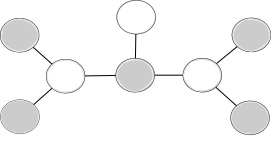
\includegraphics[scale=0.6]{images/greedy_fail.png}
	\caption{Greedy (5 nodos)}
\end{subfigure}
\begin{subfigure}[b]{0.4\textwidth}
	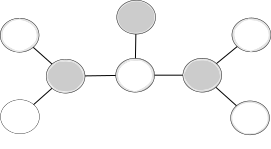
\includegraphics[scale=0.6]{images/greedy_best.png}
	\caption{Óptimo (3 nodos)}
\end{subfigure}

\begin{subfigure}[b]{0.4\textwidth}
	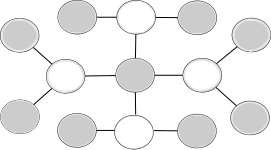
\includegraphics[scale=0.6]{images/greedy_fail2.png}
	\caption{Greedy (9 nodos)}
\end{subfigure}
\begin{subfigure}[b]{0.4\textwidth}
	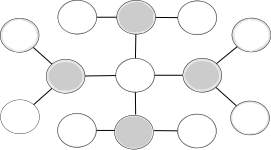
\includegraphics[scale=0.6]{images/greedy_best2.png}
	\caption{Óptimo (4 nodos)}
\end{subfigure}
\caption{Ejemplos de nuestra heurística comparado con el óptimo.}
\end{figure}

El peor caso es claramente el de la figura (c) y (d). Tenemos un nodo $v$ (el nodo central) de grado $d(v) = 4$, con sus nodos adyacentes de grado $d(u) = 3$. Si tenemos $c$ componentes conexas de ese tipo, utilizaremos $c \times (2 \times 4 + 1)$ nodos, cuando en realidad el optimo tiene $c \times 4$ nodos.



